
% !TEX root = marvin.tex
% \cleardoublepage
\clearpage
\appendix

% !TEX root = marvin.tex
\begin{figure*}[t]
  \begin{center}
  \iflatexml
  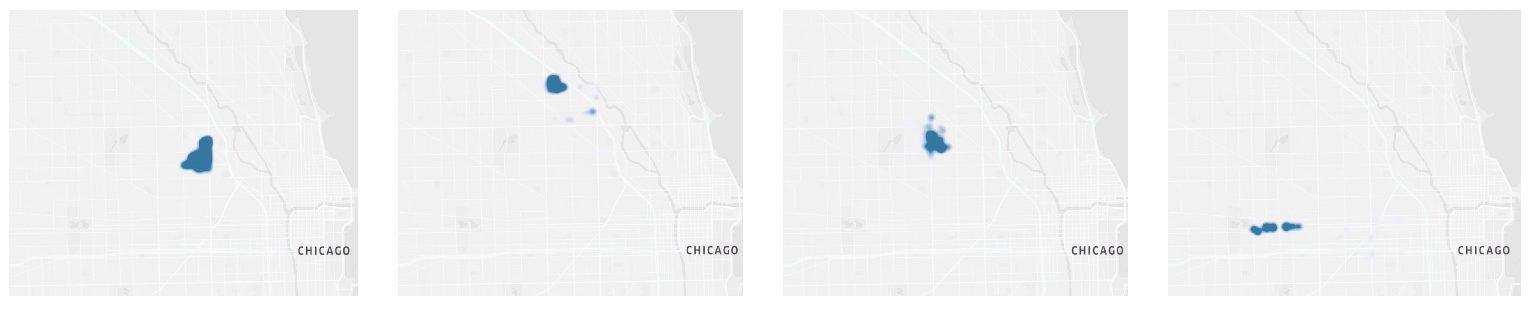
\includegraphics[width=6\textwidth]{figs/heatmap_cluster.png}
  \else
    \begin{tabular}{llll}
      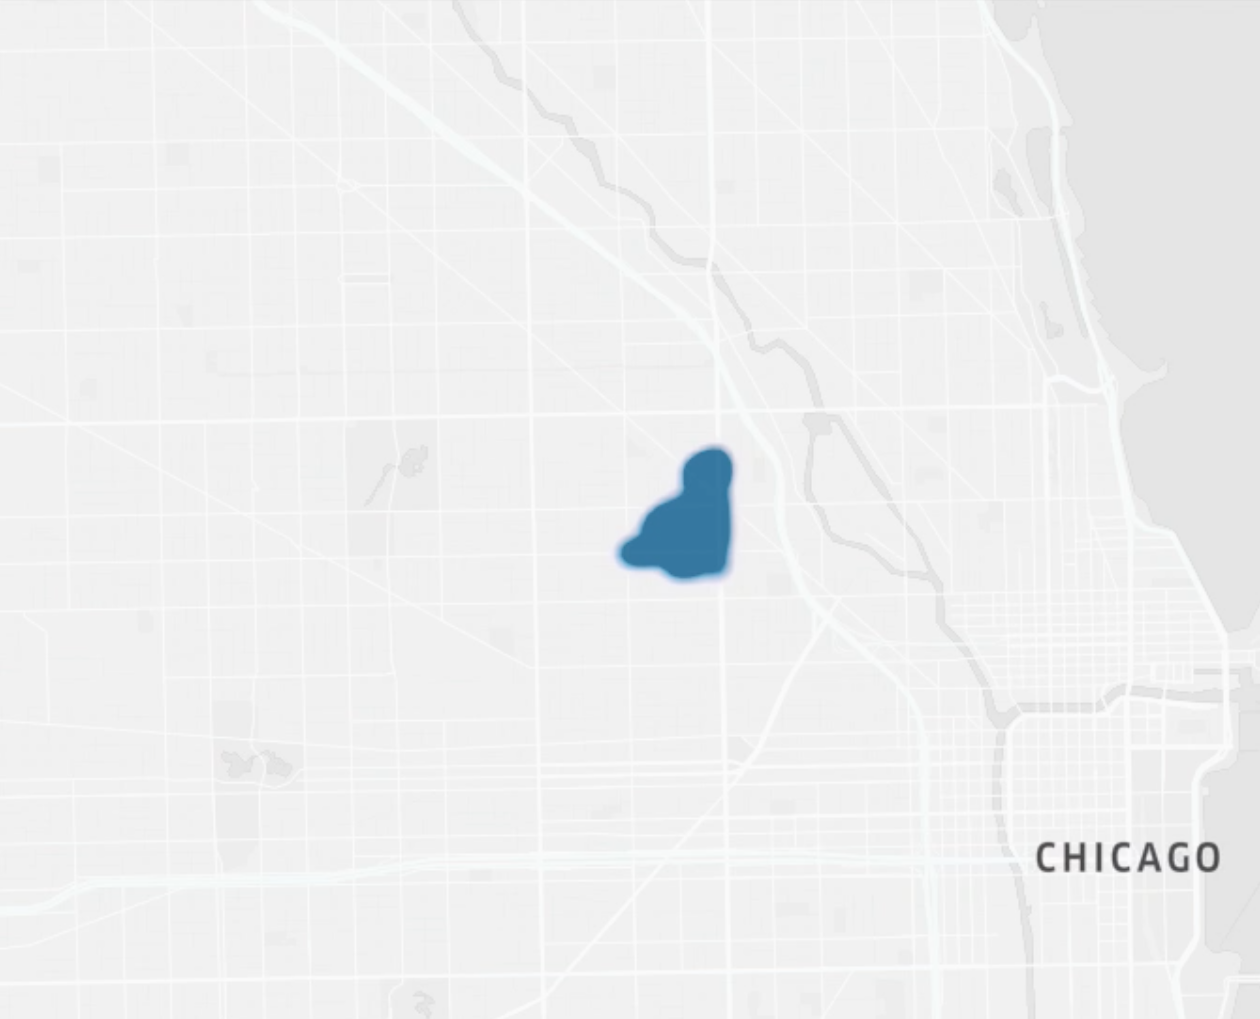
\includegraphics[height=3.0cm,trim={0.2cm 0 0.4cm 0},clip]{figs/clustered1.png} &
      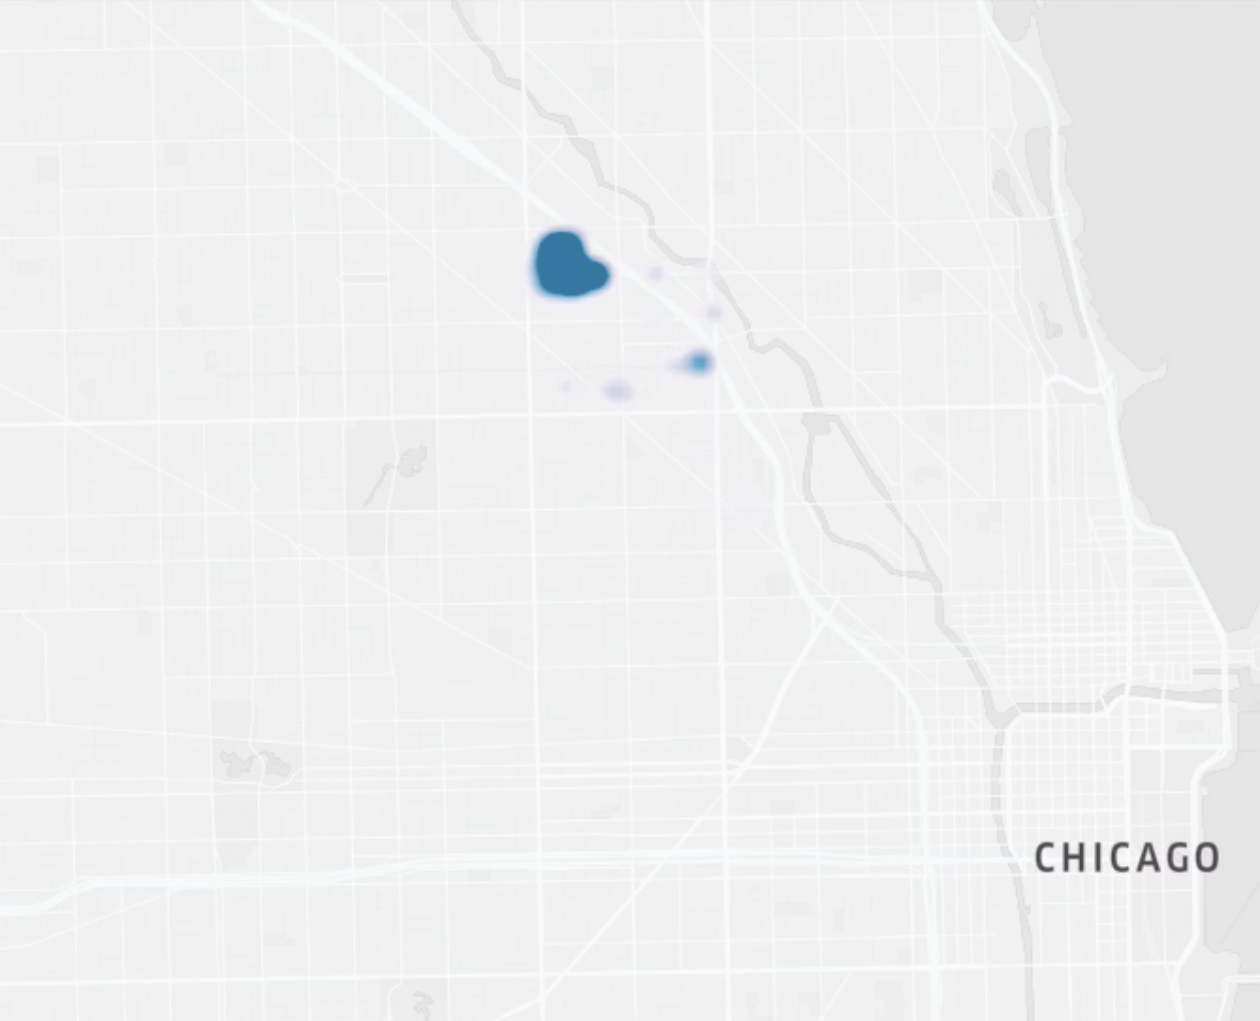
\includegraphics[height=3.0cm,trim={0.2cm 0 0.8cm 0},clip]{figs/clustered2.png} &
      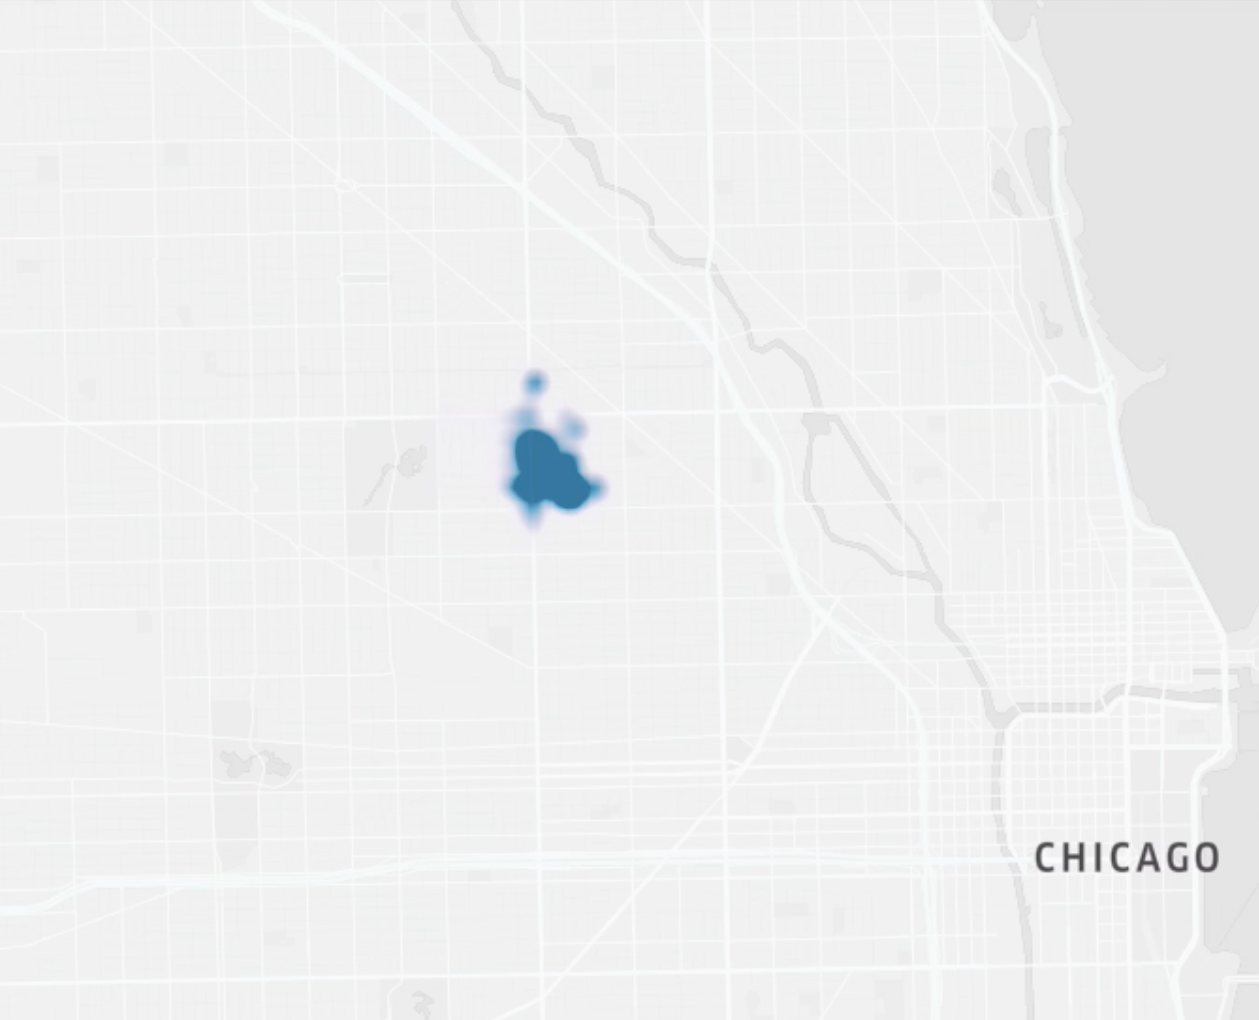
\includegraphics[height=3.0cm,trim={0.2cm 0 0.8cm 0},clip]{figs/clustered3.png} &
      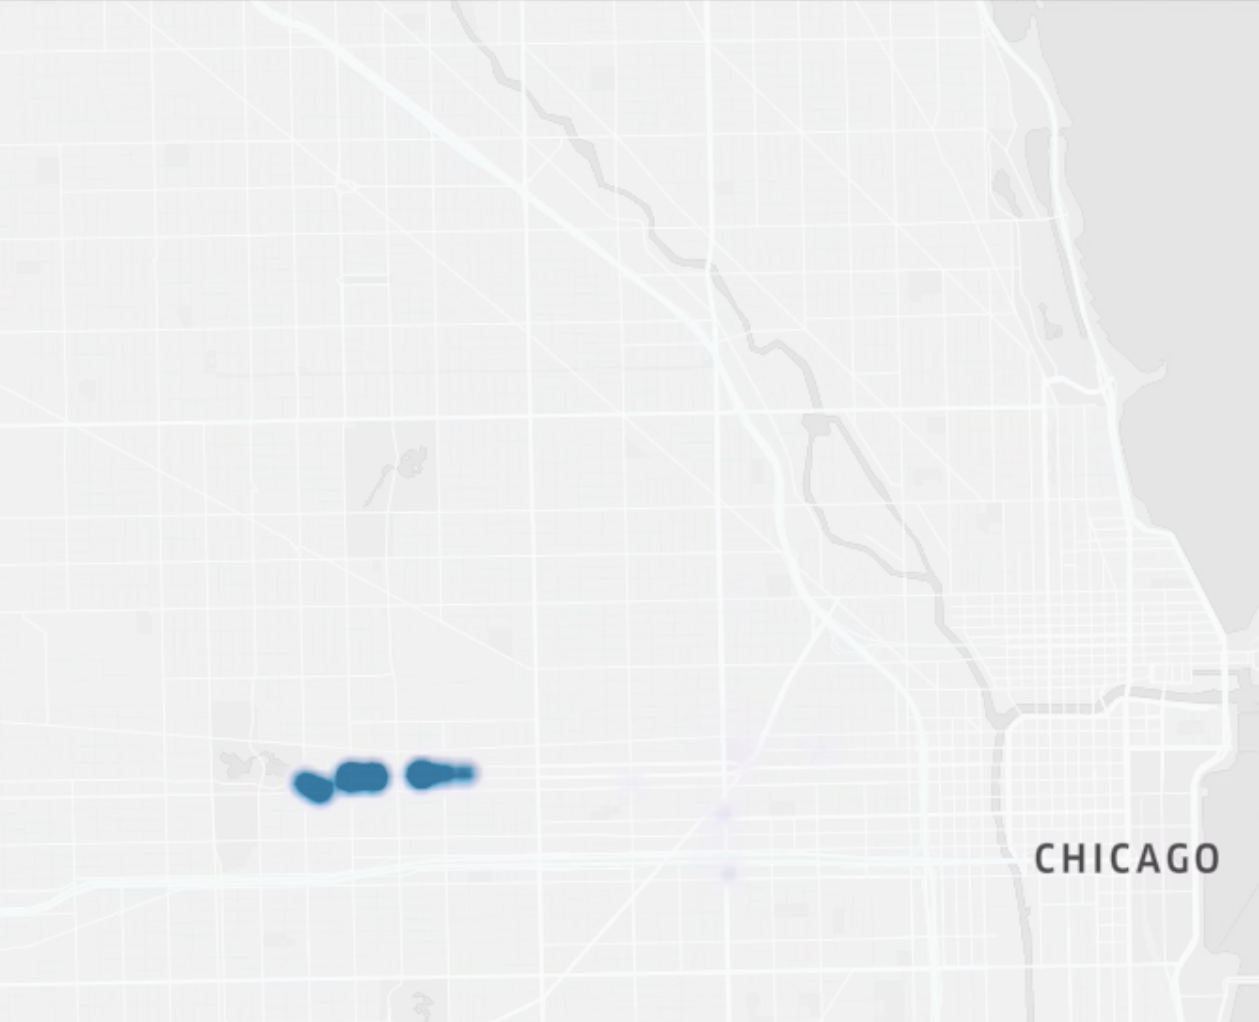
\includegraphics[height=3.0cm,trim={0.0cm 0 0cm 0},clip]{figs/clustered4.png} \\
    \end{tabular}
  \fi
  % \vspace{-0.15in}
  \caption{Value function of an agents while mapping a given region.
  The value function is high around the roads that are close
  to the agent in a sense that implies that this cluster has been
  assigned to that agent. The red dot on the left and the blue dot
  on the right represent the agent's current position.}
  \label{fig:heatmap_cluster}
  \end{center}
  \vspace{-0.25in}
\end{figure*}

% !TEX root = marvin.tex
\begin{figure*}[t]
  \begin{center}
  \iflatexml
    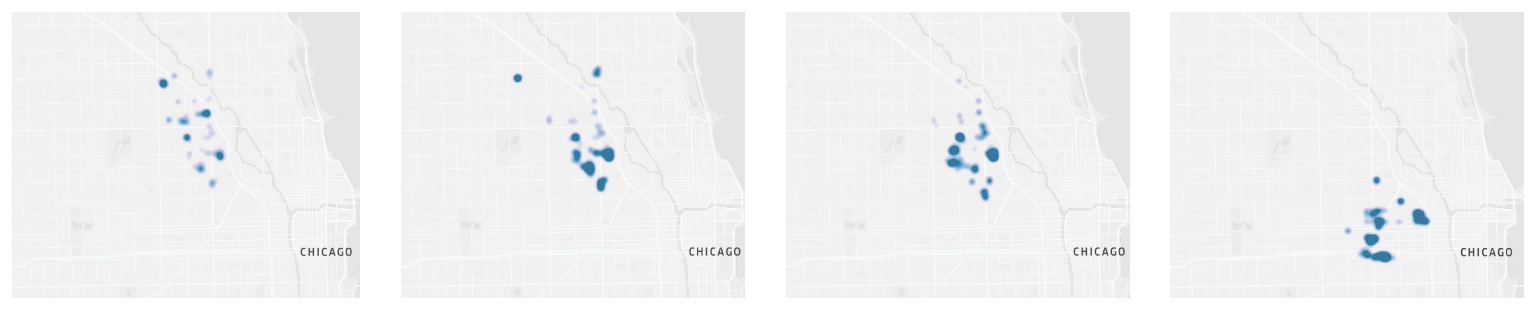
\includegraphics[width=6\textwidth]{figs/heatmap_spo.png}
  \else
    \begin{tabular}{llll}
      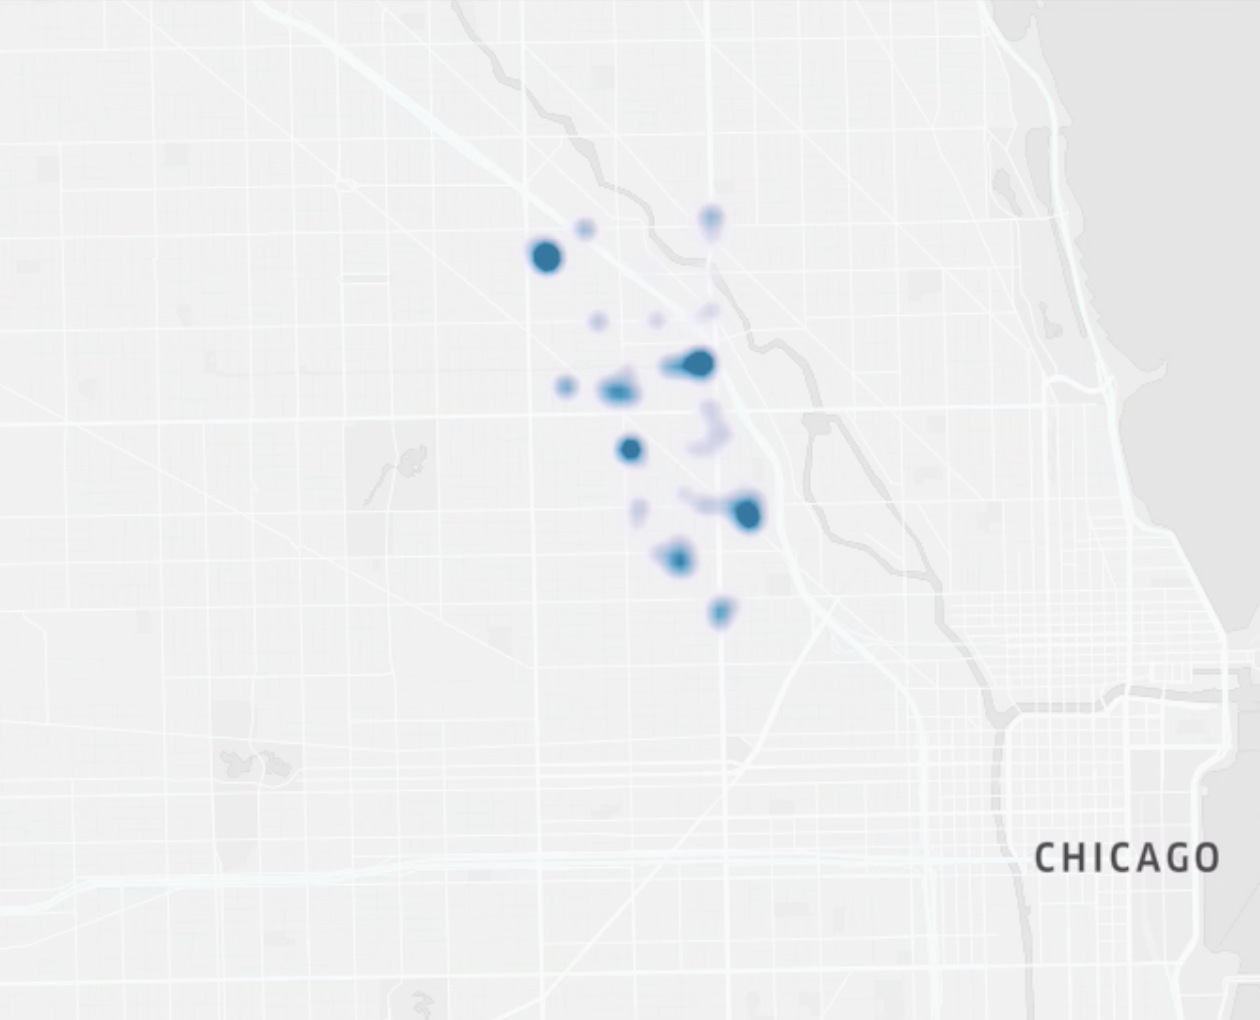
\includegraphics[height=3.0cm,trim={0.2cm 0 0.4cm 0},clip]{figs/sporadic1.png} &
      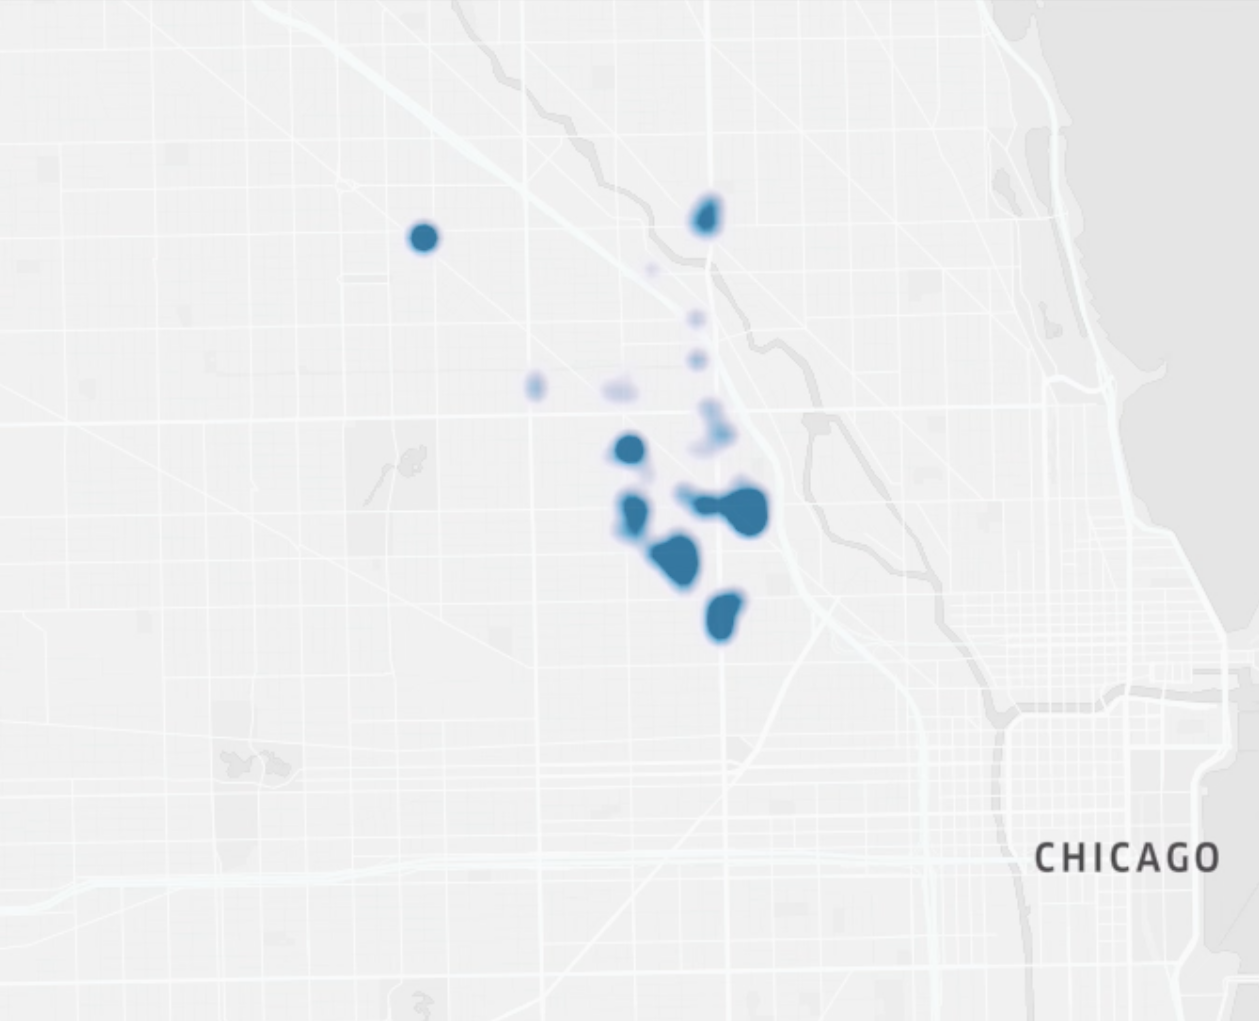
\includegraphics[height=3.0cm,trim={0.2cm 0 0.8cm 0},clip]{figs/sporadic2.png} &
      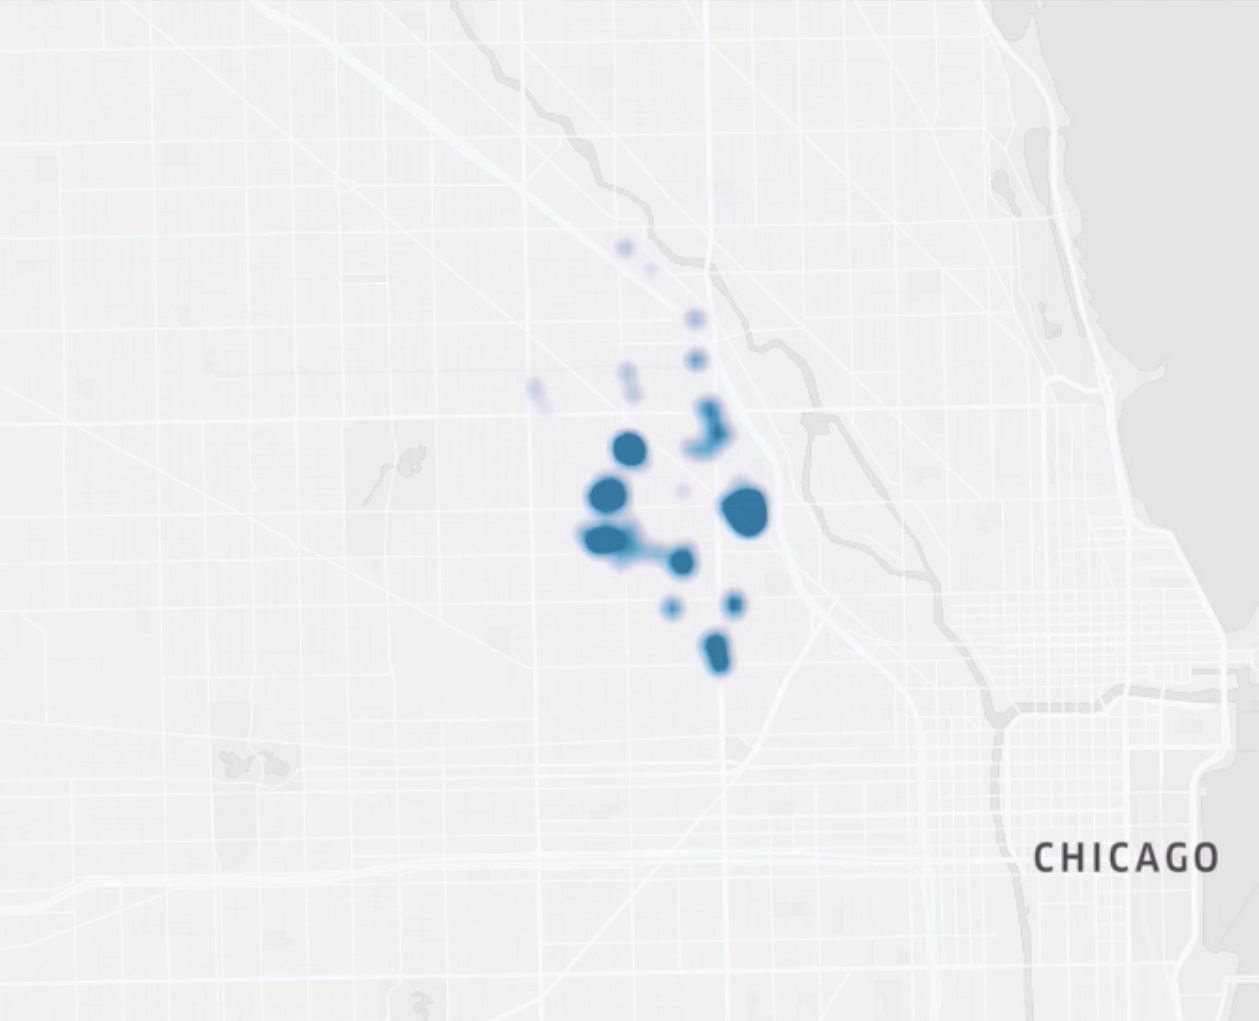
\includegraphics[height=3.0cm,trim={0.2cm 0 0.8cm 0},clip]{figs/sporadic3.png} &
      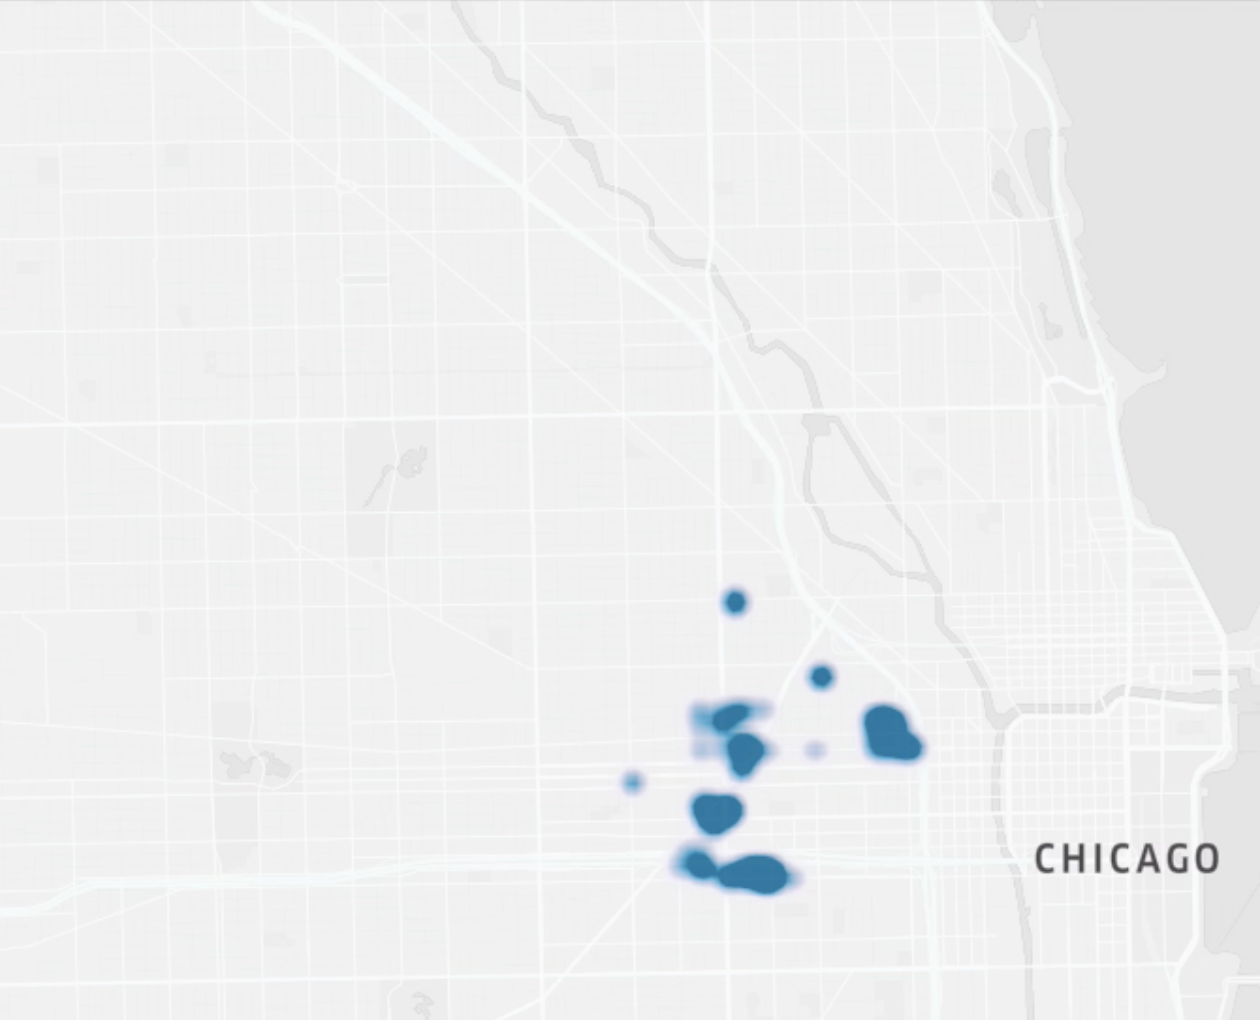
\includegraphics[height=3.0cm,trim={0.0cm 0 0cm 0},clip]{figs/sporadic4.png} \\
    \end{tabular}
  \fi
  % \vspace{-0.15in}
  \caption{Value function of an agents while mapping a given region.
  The value function is high around the roads that are distant and sporadically
  distributed implying an exploratory strategy. The red dot on the left and the blue dot
  on the right represent the agent's current position.}
  \label{fig:heatmap_sporadic}
  \end{center}
  \vspace{-0.25in}
\end{figure*}

\section{Model Action Visualization}

We firstly perform a qualitative analysis as to what kind of decisions each agent makes, and what
these decisions look like at the value function level. We then we visualize the paths that a fleet of
agents takes when mapping a large portion of Chicago from a bird's-eye-view perspective. We use this to
again qualitatively compare the strategies exploited by MARVIN trained with RL, MARVIN trained with IL,
and the GVIN.

\subsection{Value Function Heat Map}

Upon performing an analysis of the value function, we find that two main behaviors are observed. The
first is that the agent localizes the highest points in its value function to a small region of
unvisited streets. This is equivalent to having this small cluster assigned to the agent
by the collective swarm, and then it sequentially visiting all the streets until they recieve a new
objective or finish with this cluster, as can be see in Figure~\ref{fig:heatmap_cluster}.


The secondary observed behavior, as seen in Figure~\ref{fig:heatmap_sporadic}, is that the agents
occasionally begin increasing their value function at far away nodes. This can be interpreted
as the exploration phase, where the agents are encouraged to travel longer
distances in order to reach new subclusters that need to be
mapped. The peaks of the value function also appear to be relatively sporadic, indicating the
ability of the agents to consider a wide variety of potential routes.


\subsection{Overall Swarm Strategy}

We qualitatively compare our model's overall strategy to that of the generalized value iteration
network (GVIN) and observe that in general, the GVIN network tends to promote exploration.
We also observe that this high level strategy fails to cover all streets in a reliable
manner. There are small sections throughout the graph that remain unvisited, and
in order to perform a full traversal the agents must eventually
return to these small unvisited sections, often covering significant distances in
the process. This stands in contrast to what we observe with MARVIN, where the network prioritizes
covering each street in a region before moving on to the next area. This ultimately results in less
of a need for revisited regions that have incomplete mapping.

% !TEX root = marvin.tex
\begin{figure*}[t]
  \begin{center}
  \iflatexml
  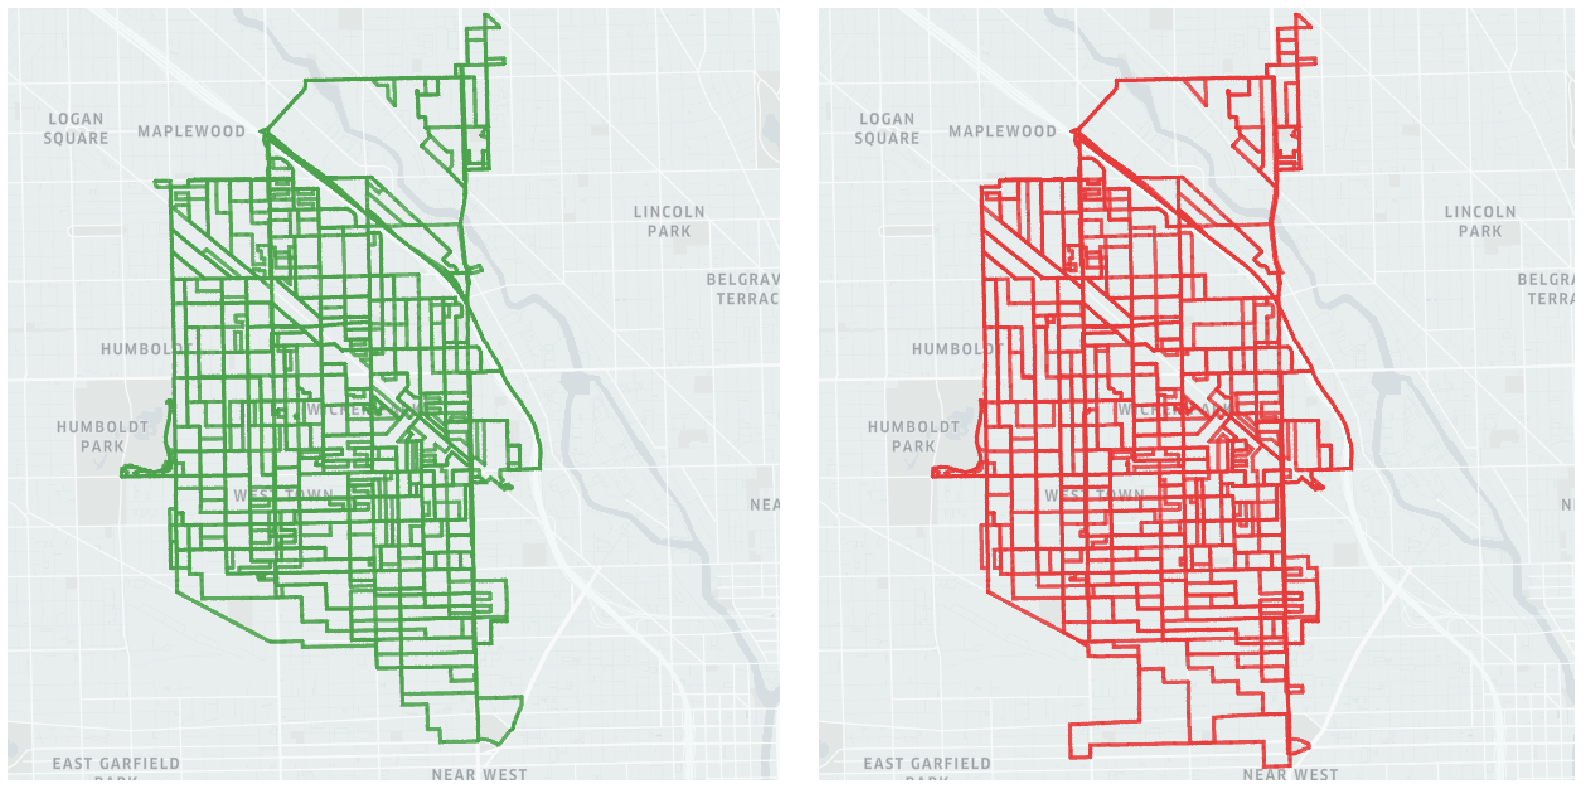
\includegraphics[width=6\textwidth]{figs/vin_gvin_all.png}
  \else
    \begin{tabular}{ll}
      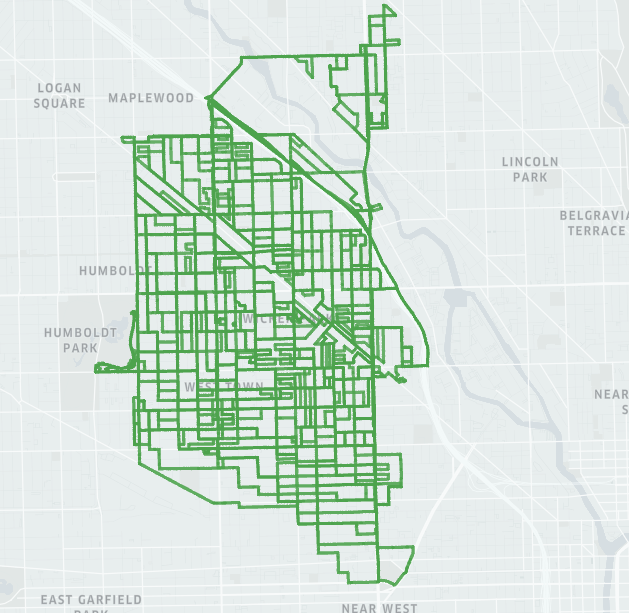
\includegraphics[height=8.1cm,trim={0.2cm 0 0.4cm 0},clip]{figs/vin_gvin_vin.png} &
      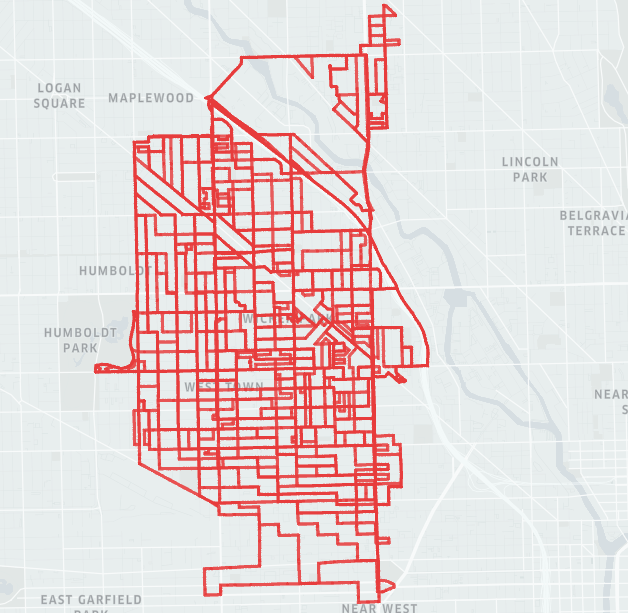
\includegraphics[height=8.1cm,trim={0.2cm 0 0.8cm 0},clip]{figs/vin_gvin_gvin.png} \\
    \end{tabular}
  \fi
  % \vspace{-0.15in}
  \caption{Bird's eye view of a partially complete traversal
  of MARVIN (left) and of the GVIN (right). While slightly more
  spread out, the traversal of the GVIN leaves many small streets
  unvisited and is less thorough overall.}
  \label{fig:vin_gvin}
  \end{center}
\end{figure*}

Next, we compare the high level strategy of MARVIN when trained with reinforcement learning to that
when trained with imitation learning. We observe that in this context, both methods prioritize a
thorough traversal, but that the agents trained using imitation learning are more efficient and
therefore are able to expand to new regions much quicker than the agents trained with reinforcement
learning. This matches the trend we noted when comparing training procedures and the scalability of
the models that they produce.

% !TEX root = marvin.tex
\begin{figure*}[t]
  \begin{center}
  \iflatexml
  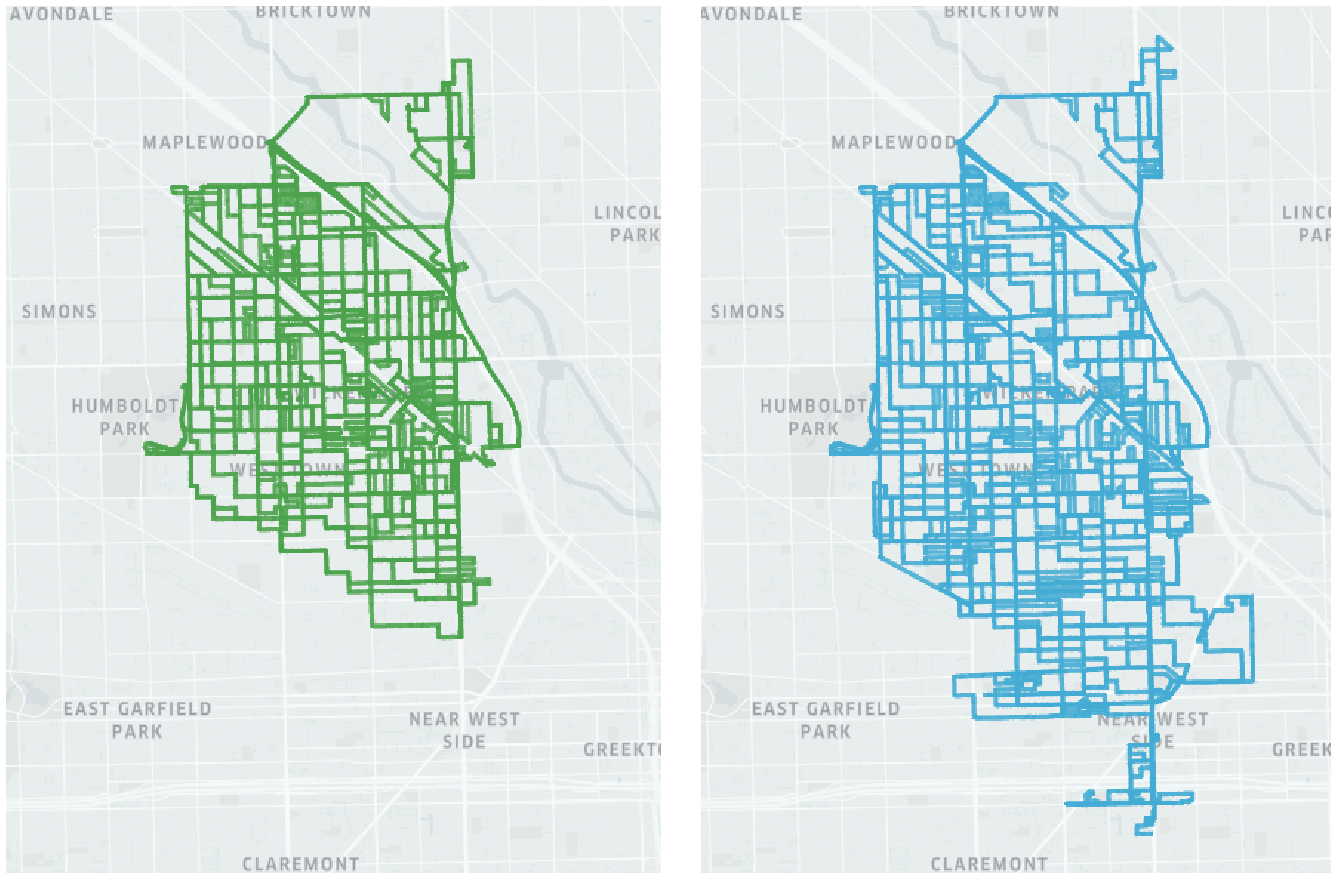
\includegraphics[width=6\textwidth]{figs/il_rl_all.png}
  \else
    \begin{tabular}{ll}
      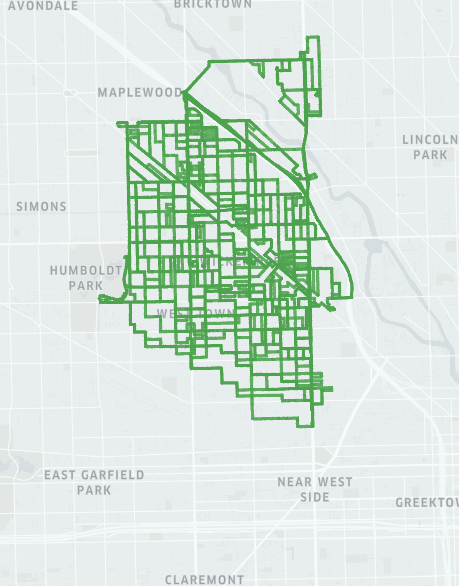
\includegraphics[height=9.1cm,trim={0.2cm 0 0.4cm 0},clip]{figs/il_rl_rl.png} &
      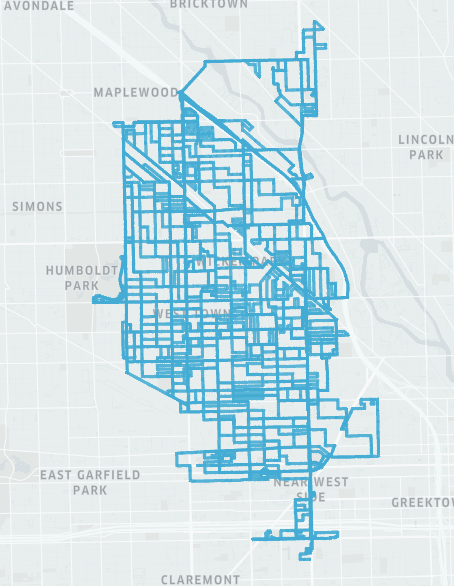
\includegraphics[height=9.1cm,trim={0.2cm 0 0.8cm 0},clip]{figs/il_rl_il.png} \\
    \end{tabular}
  \fi
  % \vspace{-0.15in}
  \caption{Bird's eye view of a partially complete traversal
  of MARVIN trained with RL (left) and MARVIN trained with IL
  (right). Both are relatively thorough while expanding to new
  regions, but the model trained using imitation learning is
  able to cover the regions in a more efficient manner.}
  \label{fig:il_rl}
  \end{center}
\end{figure*}

\section{Sample Graph Visualization}

We visualize a few of the graphs that are used in the training process seen in Figure \ref{fig:example_graphs}.
While each one can be represented by a strongly connected graph, they nevertheless posess distinct
features which enable a higher degree of generalization during the training process.

% !TEX root = marvin.tex
\begin{figure*}[t]
  \begin{center}
  \iflatexml
  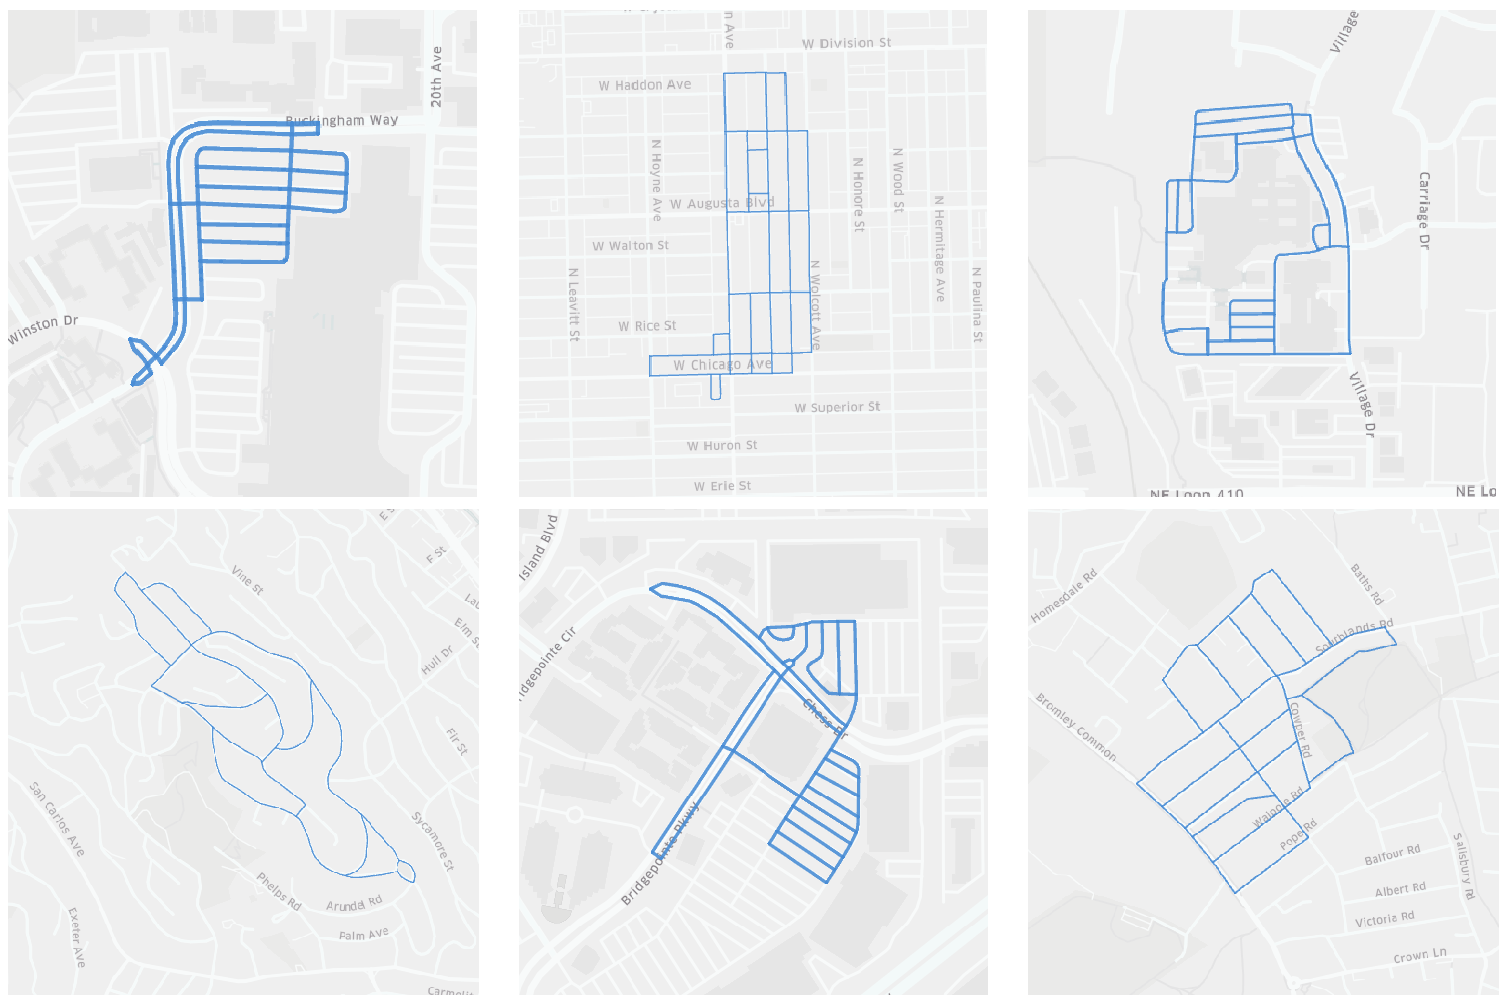
\includegraphics[width=6\textwidth]{figs/example_graphs.png}
  \else
  \begin{tabular}{lll}
    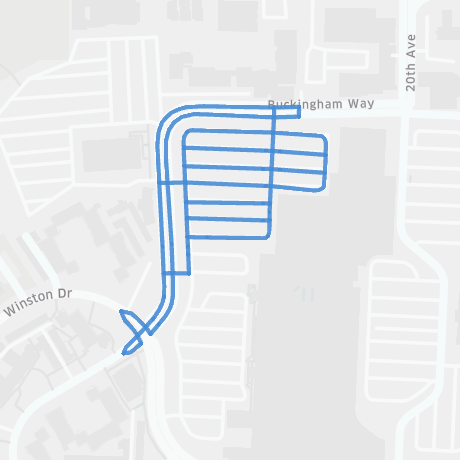
\includegraphics[height=5.1cm,trim={0.2cm 0 0.4cm 0},clip]{figs/graph1.png} &
    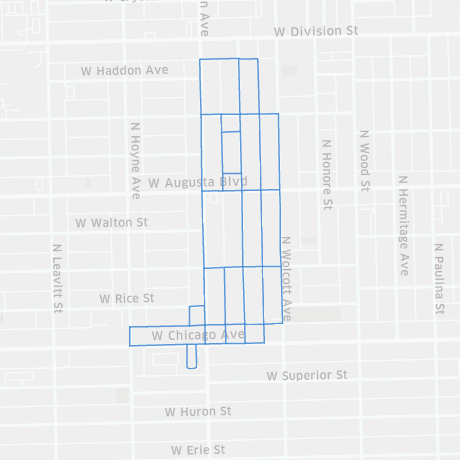
\includegraphics[height=5.1cm,trim={0.2cm 0 0.4cm 0},clip]{figs/graph2.png} &
    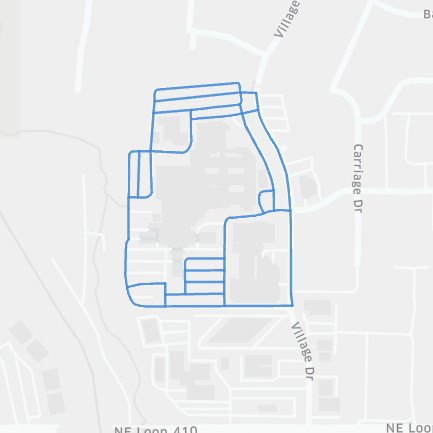
\includegraphics[height=5.1cm,trim={0.2cm 0 0.4cm 0},clip]{figs/graph3.png} \\
    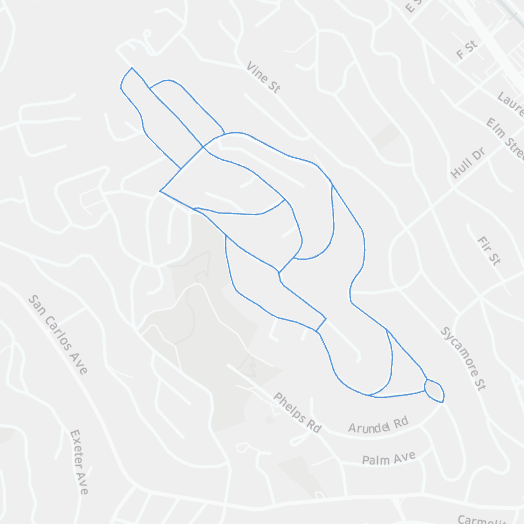
\includegraphics[height=5.1cm,trim={0.2cm 0 0.4cm 0},clip]{figs/graph4.png} &
    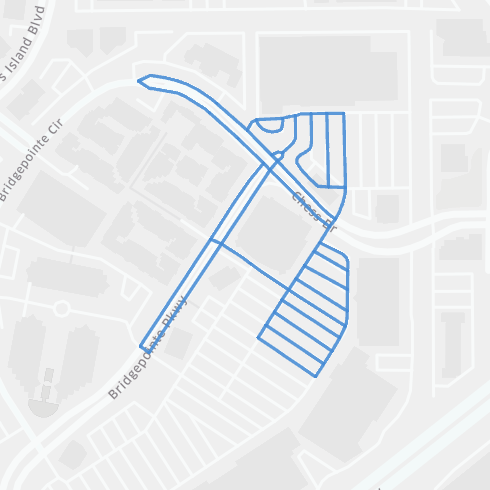
\includegraphics[height=5.1cm,trim={0.2cm 0 0.4cm 0},clip]{figs/graph5.png} &
    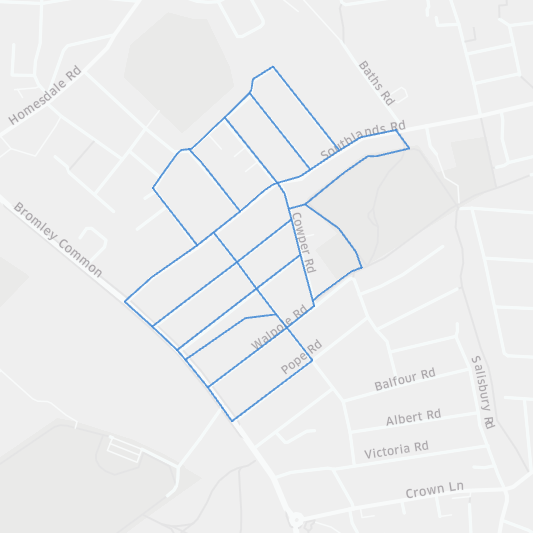
\includegraphics[height=5.1cm,trim={0.2cm 0 0.4cm 0},clip]{figs/graph6.png} \\
  \end{tabular}
  \fi
  % \vspace{-0.15in}
  \caption{Random graphs sampled from the training set. }
  \label{fig:example_graphs}
  \end{center}
  \vspace{-0.25in}
\end{figure*}